Медленное многообразие для системы (\ref{fullt}) представляет собой множество:
$$M_0 = \{(x, y, \lambda, \Lambda): \Lambda = 0, u(x,y) \sin \lambda = v(x,y) \cos \lambda \}.$$

Заметим, что выражение $\lambda = \arctan \big( \frac{v}{u} \big) + \pi k$ удовлетворяет условию $u \sin \lambda = v \cos \lambda$ для произвольных целых $k$. Однако, данное семейство функций терпит разрыв при переходе $u$ через 0. Данную проблему можно решить, гладко сшивая эти функции при различных $k$. Принимая во внимание то, что $\lambda\in S^{1}$, получим при этом пару непрерывных функций 
\newline $\lambda_{\pm}:\mathbb{R} \setminus \{ (x,y): u(x,y) = v(x,y) = 0 \}\to S^{1}$, значения которых отличаются на $\pi$:
$$\lambda_{+}(x,y) \equiv \begin{cases} 
        \arctan \frac{v}{u},        &  u>0, v > 0, \\
        \arctan \frac{v}{u} + \pi,  &  u<0, \\
        \arctan \frac{v}{u} + 2\pi, &  u>0, v<0,
       \end{cases}
$$
$$\lambda_{-}(x,y) \equiv \begin{cases} 
        \arctan \frac{v}{u} + \pi,  &  u>0, v > 0, \\
        \arctan \frac{v}{u} + 2\pi, &  u<0, \\
        \arctan \frac{v}{u} + 3\pi, &  u>0, v<0.
       \end{cases}
$$
Таким образом, вне точек $(x,y): u(x,y) = v(x,y) = 0$ медленное многообразие представляет собой двулистную поверхность.

Отдельный вопрос составляет случай когда $u$ и $v$ одновременно обращаются в ноль. При этом условие $u \sin \lambda = v \cos \lambda$ выполняется при произвольных 
$\lambda$ и решением является пара окружностей:
$$y_b=0,\quad x_b^{\pm}=\frac{-e_JD \pm e_J \sqrt{D^2-4EC}}{2C},\quad \Lambda = 0,\quad \lambda\in S^{1}.$$

Опишем геометрию медленного многообразия вблизи этих окружностей. Для этого разложим функции $u$ и $v$ в ряд в окрестности точки $(x_{b}^{\pm}, y_{b})$:
\begin{align*}
&u = \frac{C}{4}(2x+\tilde \alpha)^2-Cy^2+K = C(x-x_b^\pm)(2x_b^\pm + \tilde \alpha) + C(x-x_b^\pm)^2 - Cy^2,\\
&v = Cy(2x+ \tilde \alpha) = Cy(2x_b^\pm + \tilde \alpha) + 2Cy(x-x_b^\pm).
\end{align*}

Тогда в главном приближении уравнение на медленное многообразие примет вид:
$$(x-x_b^\pm)\sin \lambda = y \cos \lambda.$$
Следовательно, вблизи обеих перемычек медленное многообразие локально ведет себя как винтовая поверхность $\tg\lambda = \frac{y}{x-x_{b}^{\pm}}$.
Заметим, что при полном обходе перемычки в положительном направлении $\lambda$ увеличивается на $2\pi$

\begin{figure}[H]
\centering
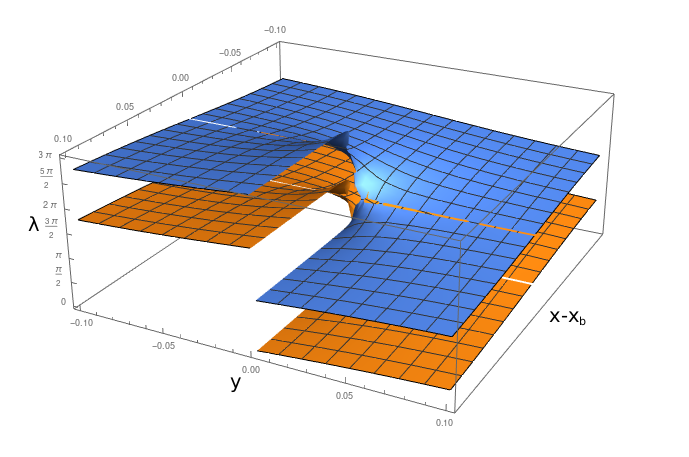
\includegraphics[scale=0.55]{img/local2.png}
\caption{Локальная струкура медленного многообразия вблизи каждой из перемычек. Разным цветом обозначены различные листы. Разрывы на каждом из листов обусловлены дефектами графопостроителя}
\end{figure}

Таким образом, мы приходим к следующему

\begin{utv}

Медленное многообразие $M_0$ плоской эллиптической ограниченной задачи трех тел в окрестности резонанса 3:1 состоит из 2 "листов"\, $M_{0,+}, M_{0,-}$, соединенных 2 "перемычками"\, $M_{0,b}^{\pm}$:
$$M_0 = M_{0,+} \cup M_{0,-} \cup M_{0,b}^{+} \cup M_{0,b}^{-},$$

\begin{eqnarray}
\nonumber
M_{0,+} = \Biggl\{ 
    \lambda = \lambda_{+}(x,y),
       \Lambda = 0,
       (x,y) \in \mathbb{R}^2 \setminus \{ (x,y): u=v=0 \}
       \Biggr\},\\
M_{0,-} = \Biggl\{ 
    \lambda = \lambda_{-}(x,y) + \pi,
       \Lambda = 0,
       (x,y) \in \mathbb{R}^2 \setminus \{ (x,y): u=v=0 \}
       \Biggr\},\\
M_{0,b}^{\pm} = \Bigl\{ y=0, x=\frac{-e_JD \pm e_J \sqrt{D^2-4EC}}{2C}, \Lambda = 0, \lambda \in S^1 \Bigr\}.
\end{eqnarray}
При этом листы $M_{0,+}, M_{0,-}$ гомеоморфны двумерной плоскости с двумя выколотыми точками, а перемычки $M_{0,b}^{\pm}$ гомеоморфны окружностям. 
\end{utv}

\begin{figure}[H]
\centering
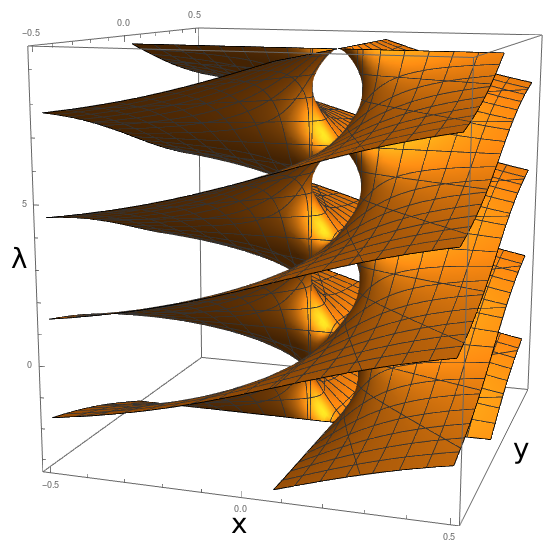
\includegraphics[scale=0.45]{img/MM.png}
\caption{Медленное многообразие}
\end{figure}

\begin{figure}[H]
\centering
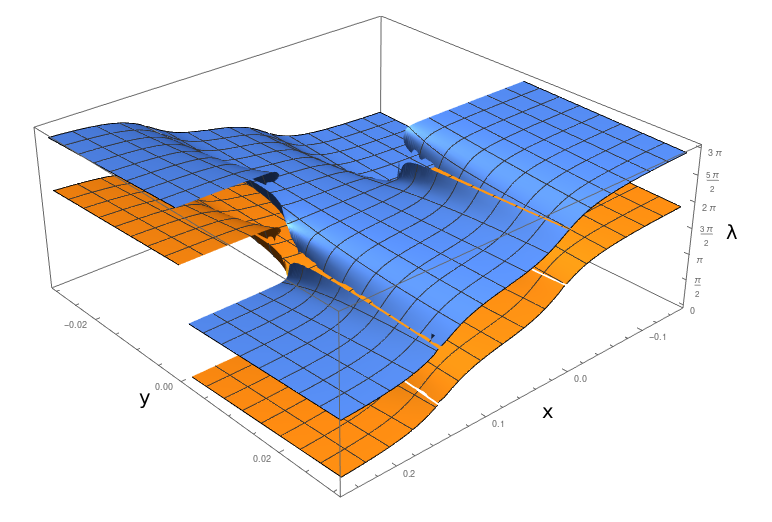
\includegraphics[scale=0.45]{img/MM2.png}
\caption{Медленное многообразие. Различным цветом обозначены различные его листы. Разрывы на каждом из листов связаны с недостатками графопостроителя}
\end{figure} 
